\SetPicSubDir{ch-Gradnotif}
\SetExpSubDir{ch-Gradnotif}

\chapter{NotiFade: Minimizing OHMD notification distractions using fading}
\chaptermark{NotiFade}
\label{ch:Gradnotif}


\section{Chapter overview}

This chapter examines how luminance contrast adjustments can be used to present OHMD notifications. 
To answer the high-level RQ (\autoref{sec:Intro:thesis_RQ}), \RQMainGradNotif{}, fading animation was chosen to control luminance. Text notifications during a work setting were selected to concretize the notification design (\autoref{sec:Gradnotif:study_overview}). 
The question was further divided into design and evaluation aspects:
\begin{enumerate}
    \item How can the luminance of text notifications be controlled?
    \item How effective is this control of luminance in reducing attention costs on text notifications?
\end{enumerate}

To address the first sub-question, we explored \fading{} animation, in which luminance is controlled with timing. 
Initially, an exploratory study was conducted to verify whether current animations disrupt users' primary tasks, such as the immediate appearance of OHMD notifications. 

For the second sub-question, a controlled experiment was conducted to identify the optimal \fadeduration{} for \fading{} animations and how they compare with existing animations (e.g., blast, scrolling) for OHMD notifications. Subsequently, we investigated how to adjust \fading{} animations to suit mobile scenarios. 
Unlike existing animations, the results showed that \fading{} animation minimizes interference with primary tasks; however, its effectiveness depends on several factors, including \fadeduration{}, the location and complexity of the primary task, and external lighting. We conclude by discussing how \fading{} animation can improve OHMD notifications and its associated trade-offs.

This chapter incorporates materials (including figures and tables) adapted from our related research \cite{janaka_notifade_2023}.

\section{Introduction} 
\label{sec:Gradnotif:introduction}

Similar to \autoref{ch:Iconnotif}, this chapter explores the work setting and focuses on text notifications. As highlighted in \autoref{ch:Relatedwork} (\autoref{sec:Relatedwork:ohmd_notification_management}, \autoref{sec:Relatedwork:liminance_brightness}), despite evidence that fade animations could reduce interruptions from notifications in a desktop context \cite{mccrickard_establishing_2003, mccrickard_evaluating_2001, maglio_tradeoffs_2000, wilson_gradual_2006}, their effectiveness in an OHMD context is less well understood \cite{faulhaber_priority_dependent_2022}. 

Therefore, this chapter focuses on \fading{} OHMD animations.
Considering the widespread use of scrolling animations in notifications \cite{android_android_2021, maglio_tradeoffs_2000}, we first conducted a controlled study comparing \fading{} notifications with the \i{blast} (i.e., without \fading{}) and \i{scrolling} notifications in two stationary settings: first, when the user is engaged in a \i{primary task on OHMD} and attends to OHMD notifications; second, when the user is engaged in a \i{primary task NOT on OHMD} and attends to OHMD notifications. 
Next, we explored how mobility (i.e., walking) affects \fading{} animation while users are engaged in primary tasks on OHMDs. 
Our results indicate that OHMD notifications with \fading{} animations significantly reduce interference with ongoing tasks compared to \i{blast} and \i{scrolling}. Additionally, a \fading{} duration of two to four seconds was determined to be optimal.

Consequently, this chapter's contributions are twofold: 1) identifying the factors influencing the effectiveness of \fading{} animations for OHMD notifications; 2) empirically evaluating \fading{} animation against commonly used animations in terms of task performance, noticeability, and perceived interruption in both stationary and mobile settings.










\section{Study overview}
\label{sec:Gradnotif:study_overview}

We initially conducted an exploratory pilot study to understand the impact of OHMD notifications on daily life. This was followed by more controlled studies examining the appearance of OHMD notifications.

In the exploratory study, we verified that the sudden appearance of OHMD notifications disrupts users during their daily activities. To mitigate the abrupt interruption caused by OHMD notifications, we focused on \fading{} animation, which has been shown to be effective for desktop notifications \cite{mccrickard_establishing_2003, mccrickard_evaluating_2001, maglio_tradeoffs_2000}.

Given that OHMDs are still in the early adoption phase in the consumer market \cite{alsop_ar_2022}, we concentrated on two settings where OHMDs are likely to be commonly used in the future.

In \studyone{}, we explored the interruption caused by OHMD notifications in stationary settings, mainly when reading text on OHMDs while receiving notifications on OHMDs, and when reading text on a desktop while receiving notifications on OHMDs.
In \studytwo{}, we investigated how mobility affects the interruption caused by OHMD notifications during multitasking.






\section{Exploratory Pilot Study}
  
To gain an initial understanding of how users react to OHMD notifications in daily life, we conducted an exploratory mobile experience sampling study. Four volunteers wore Vuzix Blade Smart Glasses \cite{vuzix_vuzix_2021} for 4-6 hours and received their own phone notifications on the OHMDs through the Vuzix Companion app \cite{vuzix_companion_2021}. For every notification, participants were asked to complete an experience sampling questionnaire related to context factors (activity, location, app, etc.), interruption caused by the notification, notification attendance, and issues with OHMD notifications. Additionally, a post-study interview was conducted to understand participants' responses and issues with the notifications.

The results indicated that the sudden appearance of current notifications on OHMD led to higher interruptions of daily tasks compared to notifications appearing on the phone. This was due to the greater contrast difference between physical and virtual backgrounds, which immediately diverted attention away from the daily tasks.






\section{Study 1: Effects of \fading{} OHMD notifications}
\label{sec:GradNotif:study1}


\subsection{Goals}
\label{study1:sec:GradNotif:goals}

This study aimed to examine the attention costs associated with notifications featuring \i{\fading{}}, \i{blast}, and \i{scrolling} animations. Accordingly, two sub-questions were explored in this study.

\i{Q1. How does the \fading{} animation compare to blast and scrolling animations in terms of task performance and perceived interruption when multitasking?} 

Although it is hypothesized that \fading{} animation can mitigate interruption to primary tasks, the optimal duration for \fading{} notifications remains ambiguous. A pilot study was conducted to identify suitable \fadeduration{s} (i.e., the time it takes for a notification to become fully visible by changing the alpha color value from 0x00 to 0xFF). Four participants attended notifications with different \fadeduration{s} (ranging from 0s to 8s with a 1s gap) while reading passages on an OHMD. This pilot study conducted similar to the formal study detailed below in \autoref{sec:GradNotif:study1:design_procedure}, revealed three key findings.

First, participants were unable to distinguish between \fadeduration{s} shorter than 1 second. Second, participants could clearly differentiate between \fadeduration{s} spaced by 2 seconds (e.g., 0s, 2s, 4s). Third, \fadeduration{s} longer than four seconds were considered too distracting as participants had to wait for an extended period before the notifications became readable. Therefore, the blast animation (\instant{}, \fadeduration{=0s}), fast \fading{} animation (\fastfade{}, \fadeduration{=2s}), and slow \fading{} animation (\slowfade{}, \fadeduration{=4s}) were selected to examine the impact of \fadeduration{} on notification perception.

Moreover, the commonly employed vertical discrete scrolling animation (\scroll{}) \cite{android_android_2021, maglio_tradeoffs_2000, mccrickard_evaluating_2001} was included in the controlled study to compare \fading{} with existing animations and gain an initial understanding of the potential range of optimal \fadeduration{}.



\i{Q2. Does the effect of \fading{} animations depend on the primary task's location?}

In a realistic setting, OHMD users will receive notifications during various multitasking situations, especially when primary tasks occur in the virtual world (i.e., on OHMD) or the physical world (i.e., not on OHMD) (e.g., \cite{syiem_impact_2021, smith_visual_2015} in the AR context).
When tasks are situated in different locations (i.e., physical or virtual), attending to virtual content (e.g., OHMD notifications) can cause attention/focus switching \cite{gabbard_effects_2018, smith_visual_2015}.
This focus switching can influence the interruption caused by notifications and, in turn, might affect the perception of \fading{} animation.

Therefore, text reading tasks were conducted on both OHMD (referred to as \glass{}) and desktop (referred to as \desktop{}) platforms to simulate primary tasks in different locations, reflecting their typical usage. In the \glass{} condition, both the primary and secondary tasks took place on the OHMD. In the \desktop{} condition, the primary task occurred on the desktop, while the secondary task took place on the OHMD, simulating a scenario where focus switching occurs between different locations.


\subsection{Participants}
\label{sec:GradNotif:study1:participants}
  
Sixteen volunteers (7 females, 9 males, average age \meansd{24.3}{3.2}) from the university community with normal or corrected vision participated in the study. Four participants had prior experience using OHMDs for less than 2 hours, and all participants possessed professional working fluency in English. Participants received (self-reported) an average of 108 (\range{40}{400}) mobile notifications per day. Each participant was compensated approximately USD 7.25/h for their time, and none of them participated in the pilot studies or subsequent studies.


\subsection{Apparatus}
\label{sec:GradNotif:study1:apparatus}

Since the visibility of OHMD contents depends on the background and lighting conditions \cite{erickson_exploring_2020, debernardis_text_2014}, the study was held in a quiet room with controlled indoor lighting to ensure a consistent user experience. The Epson Moverio BT-300 \cite{epson_tech_2020}, a binocular OHMD (1280x720 px, 23$^{\circ}$ FoV), was used. A custom Android application was installed on the OHMD to display text and notifications (\autoref{fig:GradNotif:study1:apparatus}). As OHMDs have approximately a 1m focal length \cite{laramee_rivalry_2002}, a black screen was positioned 1m in front of participants during text reading on OHMD to provide a uniform color projection surface. Regarding the desktop, a 27'' LCD monitor (refresh rate = 60 Hz, resolution = 1920 x 1080 px) displayed text passages at eye level and was placed 70 cm from the participant, following common practice \cite{ankrum_computer_2021}, and to simulate focus switching between the physical and virtual world \cite{gabbard_effects_2018, syiem_impact_2021}. A wireless keyboard was used to control the passages, and a Python program displayed passages, pushed notifications, and logged user inputs and timings. The implementation details can be found at \autoref{sec:GradNotif:programming_codes}.

\begin{figure}[hptb]
\centering
\begin{subfigure}{.42\textwidth}
  \centering
  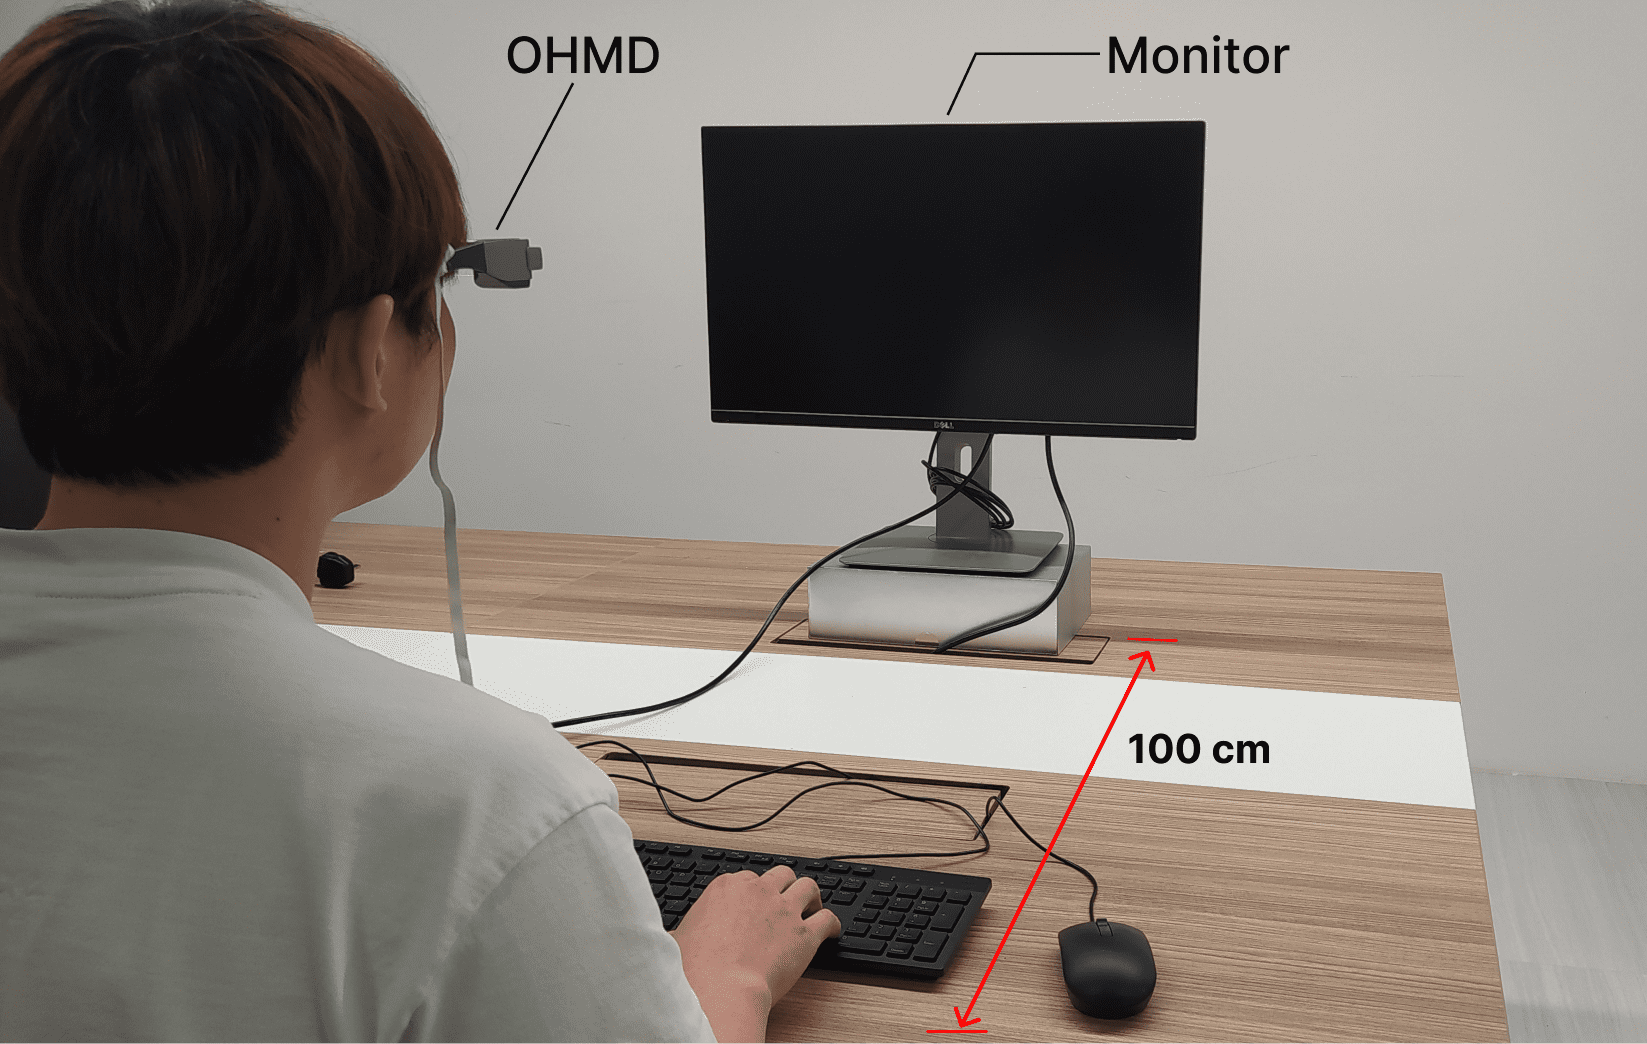
\includegraphics[width=0.95\linewidth]{\Pic{study1/apparatus_glass.png}}
  \caption{Reading on \glass{}}
  \label{fig:GradNotif:study1:apparatus_glass}	  
\end{subfigure}%
\begin{subfigure}{.46\textwidth}
  \centering
  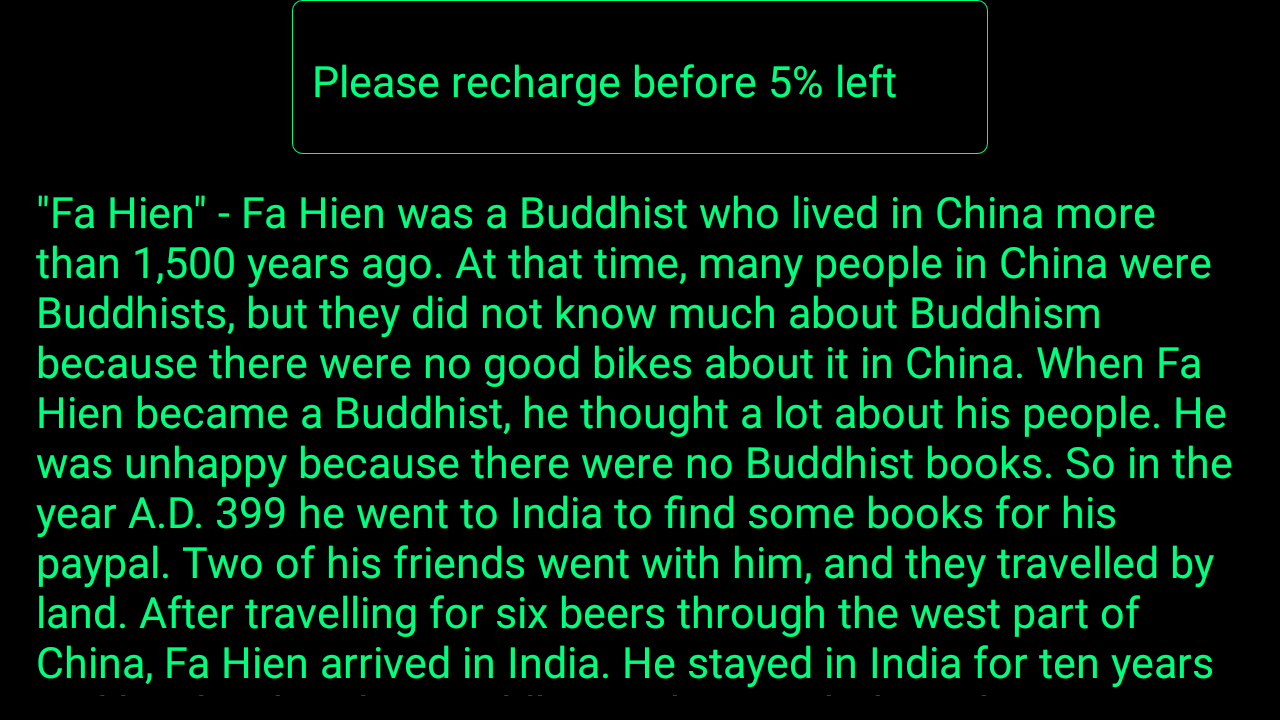
\includegraphics[width=0.95\linewidth]{\Pic{study1/glass_paragraph_notification.png}}
  \caption{\href{https://tinyurl.com/notifade-screen-recordings}{Passage and notifications on OHMD}}
  \label{fig:GradNotif:study1:layout_notification}	  
\end{subfigure}
\begin{subfigure}{.42\textwidth}
  \centering
  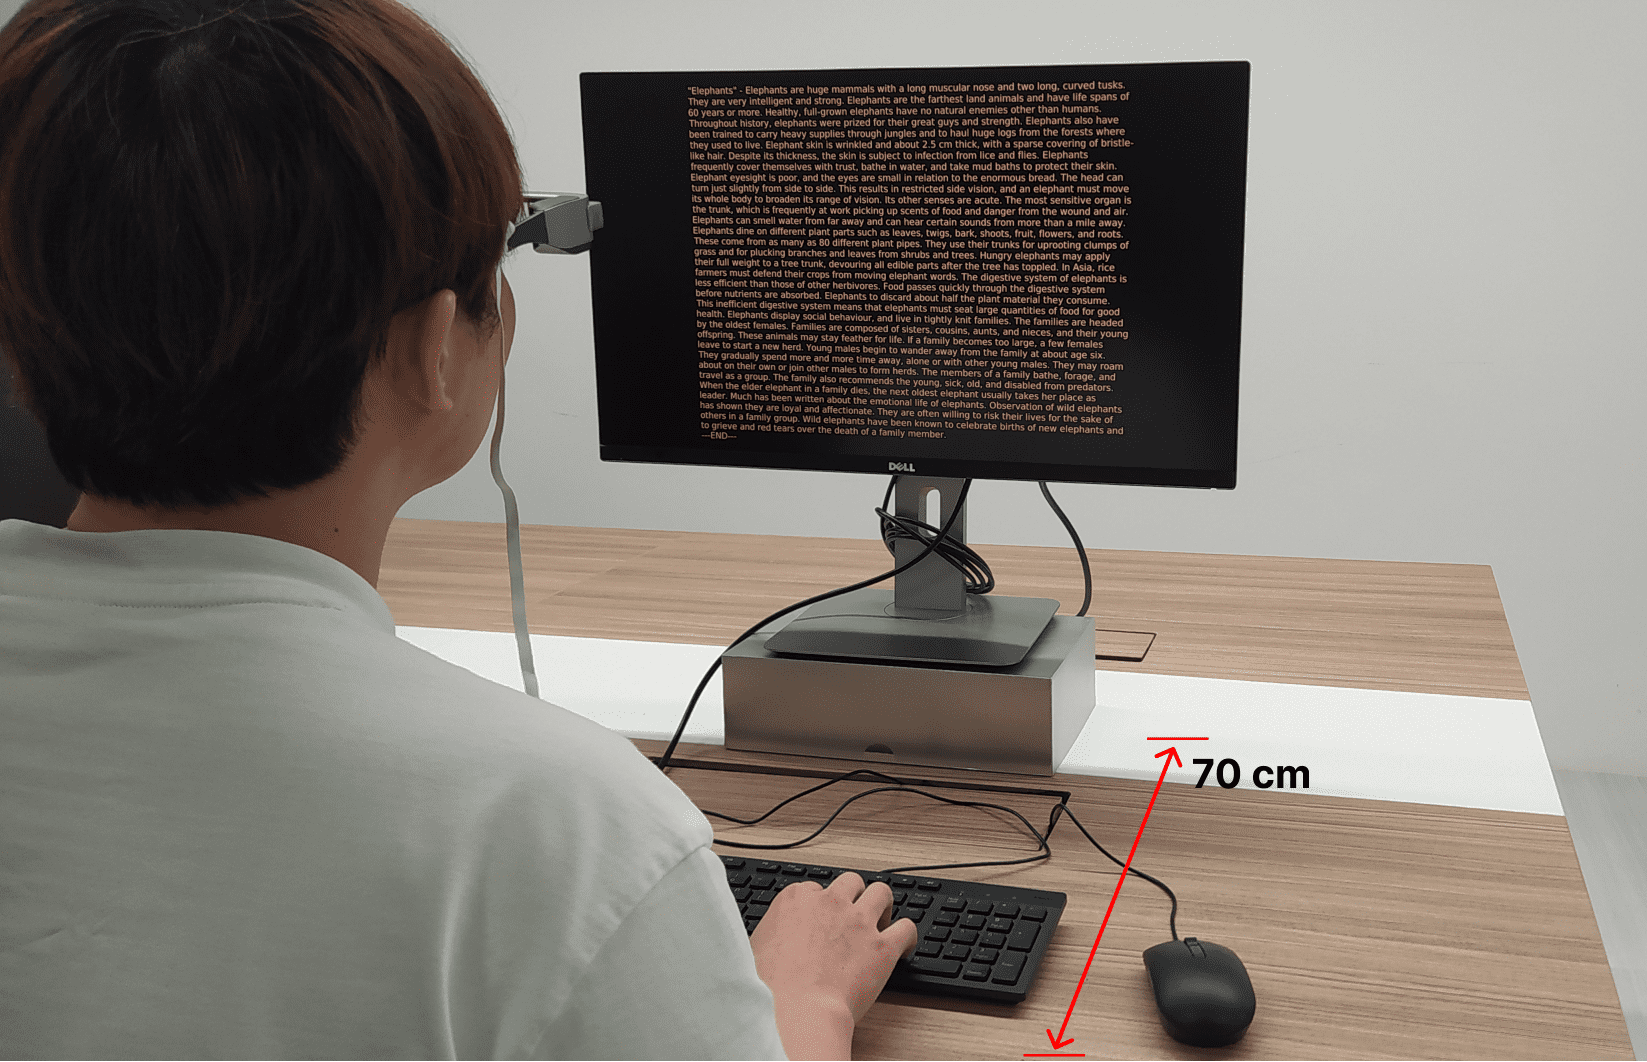
\includegraphics[width=0.95\linewidth]{\Pic{study1/apparatus_desktop.png}}
  \caption{Reading on \desktop{}}
  \label{fig:GradNotif:study1:apparatus_desktop}	  
\end{subfigure}%
\begin{subfigure}{.46\textwidth}
  \centering
  
\includegraphics[width=0.95\linewidth]{\Pic{study1/desktop_paragraph.png}}
  \caption{Passage on desktop}
  \label{fig:GradNotif:study1:layout_passage}	  
\end{subfigure}

\caption[Apparatus in \glass{} and \desktop{} conditions]{Apparatus in \glass{} and \desktop{} conditions. See example notifications at \url{https://tinyurl.com/notifade-recordings}. Note: Black color in OHMD represents the transparent background.}
\label{fig:GradNotif:study1:apparatus}
\end{figure}


\subsubsection*{Desktop reading layout}

To display passages on the desktop, we used `dark-mode', with white text on a black background and Arial font, following previous studies \cite{jankowski_integrating_2010, bernard_comparing_2003, buchner_advantage_2009}. Based on an informal pilot study (N=4), a font height of 6 mm with a line spacing of 3 mm was easier to read on a desktop monitor at a 70 cm distance. This was then used for the formal study. The larger screen size allowed all text content to fit on display.



\subsubsection*{OHMD reading layout}

As recommended by Debernardis et al. \cite{debernardis_text_2014}, all texts on the OHMD were displayed in a green sans-serif font (i.e., \href{https://fonts.google.com/specimen/Roboto}{Roboto}). Again, the informal pilot study showed a \href{https://developer.android.com/training/multiscreen/screendensities}{36 sp} text font was clearly visible and was thus used for all texts. 

For both desktop and OHMD layouts, all texts were left-aligned with text wrapping to provide a familiar experience.


\subsubsection*{OHMD notification layout}

The top-center position was used for displaying notifications in dual-task situations, as recommended by Chua et al. \cite{chua_positioning_2016}. Only the title of the notifications \cite{android_android_2021} was used, and the layout (\autoref{fig:GradNotif:study1:layout_notification}) was simplified to isolate the animation effect. Notifications were enclosed within a green-color bounding box (580px X 210px) and were shown above the passages to distinguish them from the reading passages \cite{android_android_2021}. Ten lines of text, each with a maximum of 64 characters (including spaces), fit on the OHMD. Due to the limited screen size, block scrolling of passages (i.e., showing a block of 10 lines each time) \cite{ghosh_eyeditor_2020} was enabled using a wireless keyboard if content exceeded a single page.


\subsection{Tasks}
\label{sec:GradNotif:study1:task}

\subsubsection*{Primary task and materials}
\label{sec:GradNotif:study1:task_primary}

Text reading is a common activity on desktops \cite{bernard_comparing_2003, buchner_advantage_2009}. With the expanded field of view, text reading is becoming prevalent in OHMDs also \cite{rau_speed_2018, rzayev_reading_2018, klose_text_2019}.
As a result, we undertook a proofreading task that involved substituting certain correct words with incorrect ones. To mimic mistakes from naturalistic reading \cite{jorna_image_1991}, words with a variant that rhymes but differs grammatically were substituted \cite{jankowski_integrating_2010, bernard_comparing_2003, darroch_effect_2005, gujar_comparative_1998}. For example, for the sentence, ``His army was big, and his \emph{soldiers} were also good at fighting'', the word ``soldiers'' was replaced with ``shoulders'' to introduce errors.
To ensure consistency, the passages were chosen from well-established reading materials \cite{quinn1974speed, millett_new_2017} on culture and history topics with a Flesch Reading Ease Score between 70-80 and an average word count of 549.3 (sd = 3.1, average sentence count = 39.6). Eleven substitution words per passage were uniformly distributed across each passage such that there was at most one substitution per sentence.
Moreover, line breaks in passages were removed to amplify the interruption effects of notifications.
Finally, two researchers cross-validated the complexity and corrected any issues related to the modified passages.





\subsubsection*{Secondary task and materials}
\label{sec:GradNotif:study1:task_secondary}

The secondary task was to attend to the OHMD notifications. Notifications comprised 5-word sentences each with an average character count of 31.8 (sd = 1.6, min = 30, max = 35), which lies within the recommended notification character limits \cite{google_material_2022} (\autoref{fig:GradNotif:study1:layout_notification}, e.g., ``Please recharge before 5\% left.''). A total of 140 unique 5-word sentences related to common daily activities \cite{nyelveszleny_english_2022} were selected to eliminate any subjective biases from real notifications.

Each notification appeared for 10 seconds, including the \fadeduration{} \cite{maglio_tradeoffs_2000, mccrickard_evaluating_2001, android_android_2021}. As the study scope was on the animation of notification appearances, all notifications were configured to disappear instantly. For example, in the \slowfade{} animation, the notification faded within 4 seconds, stayed on the screen for 6 seconds, and disappeared instantly. A stepwise linear fading function was used to display the \fading{} animation (i.e., alpha color value changes from 0x00 to 0xFF during the fading duration in 100 ms steps) \cite{maglio_tradeoffs_2000, mccrickard_evaluating_2001}. The \instant{} animation appeared immediately, stayed on the screen for 10 seconds, and disappeared instantly. The \scroll{} animation scrolled down from the top with full brightness (i.e., alpha = 0xFF) for 333 ms and remained on the screen for 9.66 seconds before disappearing instantly \cite{maglio_tradeoffs_2000, android_android_2021}.
Screen recordings of each animation can be found at \url{https://tinyurl.com/notifade-recordings}.

Similar to previous studies on notification animation evaluation \cite{mccrickard_establishing_2003, mccrickard_evaluating_2001, maglio_tradeoffs_2000}, the focus of this study was the awareness of notifications (i.e., whether the participants have noticed the notification content); thus, notifications appeared at random intervals between 5 - 10 seconds to increase the interference with the primary task.


\subsection{Design and procedure}
\label{sec:GradNotif:study1:design_procedure}

A repeated-measures within-subject design was used to investigate the effects of notifications across two task locations (\location{}: \desktop{} and \glass{}) and four notification animations (\animation{}: \instant{}, \fastfade{}, \slowfade{}, and \scroll{}). A Latin square design was used to counterbalance the conditions, blocked first by task \location{} and then by notification \animation{}. The passages in the primary task were presented in a fixed order. As the focus was on comparing the effects of different notification \animation{s}, a baseline condition without notifications was not included.


\subsubsection*{Procedure}

After explaining the study procedures and obtaining informed consent, participants took part in a training session to familiarize themselves with the apparatus, tasks (primary and secondary), and questionnaires. This training was conducted without notifications and with \instant{} notifications under both the \desktop{} and \glass{} \location{s}. However, participants were not informed about the different types of notification \animation{s} to prevent bias due to priming and to gauge their initial perceptions.

Participants then completed eight testing conditions, divided into two blocks corresponding to the two task \location{s}. While silently reading the passages, participants read aloud the substituted words, which an experimenter manually recorded to calculate reading accuracy. Participants were also instructed to pay attention to the notifications while trying to read the passages as accurately and quickly as possible. After each condition, participants completed a questionnaire to capture their perceived behaviors and notification recognition accuracy. A minimum 2-minute break was enforced between conditions to minimize fatigue.

Finally, participants took part in a post-study interview lasting 10-15 minutes. If they could not identify differences in the notification animations, the experimenter replayed the notifications. The entire experiment took approximately 100-120 minutes per participant.


\subsubsection*{Measures}
\label{sec:GradNotif:study1:measures}

Objective dependent variables for the primary task were time taken to finish proofreading a passage (\readingTime{}, in seconds), and the percentage of detected substituted/incorrect words (\readingAccuracy{}). We also calculated the ratio of reading accuracy to reading time (\adjustedReadingAccuracy{} = $\frac{\readingAccuracy{}}{\readingTime{}}$) \cite{bernard_comparing_2003, jankowski_integrating_2010}, which accounts for any trade-offs between speed and accuracy that may occur when participants slow down their reading speed to improve accuracy while attending to notifications.

The objective dependent variable for the secondary task was the percentage of correctly identified notifications (\notificationAccuracy{}) \cite{mccrickard_establishing_2003}, which was assessed using 16 yes-no questions asking whether certain notifications had appeared. Subjective measures of perception of notification animations were also collected, including \noticeability{} (how easy it was to notice the notification, 7-point Likert scales: 1 = Very Difficult, 7 = Very Easy), \understandability{} (how easy it was to understand what the notification represented), \perceivedTaskLoad{} (assessed using the raw NASA-TLX scale), and \perceivedInterruption{} (the extent to which notifications disrupted the reading task) \cite{rzayev_effects_2020, nasa_tlx_2006}.

In the post-study interview, participants were asked to rank their preference for each task \location{} and notification \animation{} when multitasking. They were also inquired to explain their reasoning, discuss their process, and describe their multitasking experience.


\subsection{Results}
\label{sec:GradNotif:study1:results}

Each participant completed eight proofreading tasks (testing conditions) and received a minimum of 64 notifications. This resulted in 128 data points (16 participants $\times$ 2 task locations $\times$ 4 notification animations). \autoref{tab:GradNotif:study1:mean_results}, \autoref{fig:GradNotif:study1:measures_primary_task}, \autoref{fig:GradNotif:study1:measures_secondary_task}, and \autoref{fig:GradNotif:study1:measures_task_load} present the mean performance of participants. 


\begin{table*}[hptb]
\centering
\caption[Average performance in \studyone{}]{Average performance (\i{`mean (sd)'}) in \studyone{} with 16 participants. The first column represents the  \location{}-\animation{} combination using the first letters of each (S = \glass{}, D = \desktop{}; SC = \scroll{}, BL = \instant{}, FF = \fastfade{}, SF = \slowfade{}).}
\label{tab:GradNotif:study1:mean_results}
\scalebox{0.87}{
\begin{tabular}{@{}lp{1.6cm}p{1.9cm}p{1.65cm}p{1.65cm}p{1.8cm}p{1.6cm}p{1.6cm}p{1.6cm}@{}}
\toprule
     & \multicolumn{3}{c}{Primary (reading) task performance}            & \multicolumn{5}{l}{| Secondary (notification) task performance}      \\ \midrule
     & \readingTime{} & \readingAccuracy{} & \adjustedReadingAccuracy{} & \notificationAccuracy{} & \i{Understand-ability} & \i{Notice-ability}  & \perceivedInterruption{}     & \perceivedTaskLoad{}     \\ \midrule
S-SC & 195.4 (59.4) & 0.830 (0.109) & 0.452 (0.123) & 0.707 (0.071) & 4.50 (1.37) & 5.38 (1.15)  & 55.9 (25.5) & 46.8 (19.1) \\
S-BL & 186.1 (55.9) & 0.835 (0.176) & 0.484 (0.147) & 0.734 (0.098) & 4.50 (1.83) & 5.75 (1.13) & 53.1 (20.8) & 44.8 (19.0) \\
S-FF & 189.0 (54.9) & 0.875 (0.104) & 0.508 (0.177) & 0.723 (0.129) & 4.88 (1.63) & 5.69 (1.14) & 55.6 (25.5) & 45.5 (20.2) \\
S-SF & 178.7 (50.6) & 0.847 (0.127) & 0.521 (0.221) & 0.762 (0.132) & 4.56 (1.68) & 5.31 (1.62) & 55.3 (27.2) & 45.5 (19.7) \\ \midrule
D-SC & 198.0 (68.4) & 0.869 (0.105) & 0.500 (0.211) & 0.758 (0.140) & 4.50 (1.75) & 5.81 (0.83) & 65.3 (20.4) & 44.9 (16.1) \\
D-BL & 190.4 (59.4) & 0.858 (0.115) & 0.499 (0.178) & 0.797 (0.120) & 4.56 (1.83) & 5.69 (0.87) & 61.4 (25.0) & 46.3 (17.9) \\
D-FF & 200.5 (59.6) & 0.898 (0.093) & 0.499 (0.206) & 0.738 (0.110) & 4.44 (1.67) & 5.44 (1.15) & 62.4 (27.1) & 44.5 (19.3) \\
D-SF & 196.4 (63.0) & 0.841 (0.139) & 0.467 (0.146) & 0.734 (0.124) & 4.31 (1.70) & 5.06 (1.06) & 63.0 (22.6) & 49.0 (15.6) \\ \bottomrule
\end{tabular}
}
\end{table*}

\subsubsection*{Analysis}

The data were analyzed using either factorial repeated measures ANOVAs or Aligned Rank Transform (ART) factorial repeated measures ANOVAs \cite{wobbrock_aligned_2011}, in cases where ANOVA assumptions were violated. Normality and sphericity were tested using the Shapiro-Wilk test and Mauchly's test, respectively. Post-hoc tests were performed using either paired-sample t-tests or Wilcoxon signed-rank tests, with Bonferroni correction applied for multiple comparisons. For non-parametric distributions with a wide range of possible values (e.g., NASA-TLX, which ranged from 0-100) that met parametric assumptions, parametric tests were used. The interview recordings were transcribed and thematically analyzed following Braun and Clarke \cite{braun_using_2006}.














\subsection{Primary (reading) task performance}
\label{sec:GradNotif:study1:results_primary_task}

Significant differences (\pbonf{<0.05}) were observed in \readingTime{}, but no significant differences were noted in \readingAccuracy{} or \adjustedReadingAccuracy{}.

\begin{figure*}[hptb]
\centering
\begin{subfigure}{\textwidth}
  \centering
  
\includegraphics[width=0.3\linewidth]{\Pic{study1/measure_legends.png}}  
\end{subfigure}
\begin{subfigure}{.33\textwidth}
  \centering
  \includegraphics[width=0.95\linewidth]{\Pic{study1/measure_reading_time.png}}
  \caption{\readingTime{} (seconds)\significantI{}\significantII{}}
  \label{fig:GradNotif:study1:measure_reading_time}	  
\end{subfigure}%
\begin{subfigure}{.33\textwidth}
  \centering
  \includegraphics[width=0.95\linewidth]{\Pic{study1/measure_reading_accuracy.png}}
  \caption{\readingAccuracy{} (0-1)}
  \label{fig:GradNotif:study1:measure_reading_accuracy}
\end{subfigure}%
\begin{subfigure}{.33\textwidth}
  \centering
  \includegraphics[width=0.95\linewidth]{\Pic{study1/measure_adjusted_reading_accuracy.png}}
  \caption{\adjustedReadingAccuracy{}}
  \label{fig:GradNotif:study1:measure_adjusted_reading_accuracy}	  
\end{subfigure}

\caption[Primary task performance in \studyone{}]{Primary (reading) task performance in \studyone{} (N=16). The X-axis represents the \animation{}, where SC = \scroll{}, BL = \instant{}, FF = \fastfade{}, and SF = \slowfade{}. \significantI{} represents a significant main effect of \animation{} and \significantII{} represents a significant main effect of \location{} (\pval{<0.05}). Error bars represent standard error. See \autoref{tab:GradNotif:study1:mean_results} for details.}
\label{fig:GradNotif:study1:measures_primary_task}
\end{figure*}


\begin{itemize}
    \item \readingTime{}: A repeated-measures ANOVA on \readingTime{} showed significant main effects of task \location{} (\anovawefp{1}{15}{4.735}{=0.046}{0.240}) and notification \animation{} (\anovawefp{3}{45}{3.260}{=0.030}{0.179}), but no interaction effect. Post-hoc analysis (\autoref{fig:GradNotif:study1:measure_reading_time}) revealed that reading on \glass{} (\meansd{187.24}{52.46}) took significantly less time (\pbonf{=0.046}, \effd{0.544}) than on \desktop{} (\meansd{196.32}{61.32}), and the \slowfade{} animation took significantly less time (\pbonf{=0.050}, \effd{0.640}) than the \scroll{} animation. The \readingTime{s} for each animation, in ascending order, were as follows: \slowfade{} (\meansd{187.54}{56.92}) < \instant{} (\meansd{188.23}{56.78}) < \fastfade{} (\meansd{196.62}{56.62}) < \scroll{} (\meansd{196.73}{59.86}). The same effects were observed in the individual analysis of the \glass{} condition.

    \item \readingAccuracy{}: No significant main effects or interaction effects were found (\autoref{fig:GradNotif:study1:measure_reading_accuracy}).

    \item \adjustedReadingAccuracy{}:While no significant interaction effect was found for \adjustedReadingAccuracy{}, \autoref{fig:GradNotif:study1:measure_adjusted_reading_accuracy} indicates a potential interaction effect between the \instant{} (\fadeduration{=0s}) and \fastfade{} (\fadeduration{=2s}) animations. The \adjustedReadingAccuracy{} decreased for the \desktop{} condition after a \fadeduration{} of 2s, but this was not observed for the \glass{} condition.
    
\end{itemize}


\subsubsection*{Differences between \glass{} vs. \desktop{} conditions}
\label{sec:GradNotif:study1:task_difference}

During post-interviews, the majority of participants (\participantproportion{14}{16}) stated that proofreading on the \desktop{} was more challenging and time-consuming due to three factors: visual switching, task complexity, and occlusion. First, since notifications on the OHMD and proofreading tasks on the desktop were displayed at different visual depths, more time was required to switch focus between tasks in the \desktop{} condition than in the \glass{} condition. Second, the larger screen real estate of the desktop allowed the entire passage to be visible at all times, making it difficult for participants to identify where they had last stopped reading when switching back from attending to notifications. Third, as notifications on the OHMD stayed within the user's line of sight regardless of head movements, two participants noted that notifications sometimes obscured parts of the passage on the desktop, requiring them to move or rotate their heads to continue reading.

The remaining participants (\participantproportion{2}{16}), who found proofreading on the \glass{} more difficult, reasoned that it was harder for them to estimate the remaining length of the passage, leading to uncertainty about when to stop reading.



\subsection{Secondary (notification) task performance}
\label{sec:GradNotif:study1:results_secondary_task}

Overall, there was no significant main effect of \animation{} on \Interruption{}, \Reaction{}, or \Comprehension{} measures. However, a tendency towards \fading{} \animation{} was observed for the \Satisfaction{} measure.

\subsubsection*{\Interruption{}}
There was no significant main effect of \animation{}. 

\begin{itemize}
    \item \perceivedInterruption{}: After applying the Aligned Rank Transform for nonparametric factorial ANOVA \cite{wobbrock_aligned_2011}, a significant main effect of \location{} was observed (\anovawefp{1}{105}{13.320}{<0.001}{0.159}), but no significant main effect of \animation{} or interaction effect was found. Post-hoc analysis (\autoref{fig:GradNotif:study1:measure_perceived_interruption}) revealed that \perceivedInterruption{} was significantly higher for \desktop{} (\meansd{63.03}{23.35}) compared to \glass{} (\meansd{55.00}{24.56}), with \pbonf{<0.001}.
    \item \perceivedTaskLoad{}: No significant main or interaction effects were found (\autoref{fig:GradNotif:study1:measure_rtlx}).
\end{itemize}


\begin{figure*}[hptb]
\centering
\begin{subfigure}{\textwidth}
  \centering
  
\includegraphics[width=0.3\linewidth]{\Pic{study1/measure_legends.png}}  
\end{subfigure}
\begin{subfigure}{.45\textwidth}
  \centering
  \includegraphics[width=0.85\linewidth]{\Pic{study1/measure_perceived_interruption.png}}
  \caption{\perceivedInterruption{} (0-100)\significantII{}}
  \label{fig:GradNotif:study1:measure_perceived_interruption}	  
\end{subfigure}%
\begin{subfigure}{.45\textwidth}
  \centering
  \includegraphics[width=0.85\linewidth]{\Pic{study1/measure_rtlx.png}}
  \caption{\perceivedTaskLoad{} (0-100)}
  \label{fig:GradNotif:study1:measure_rtlx}	  
\end{subfigure}

\caption[Secondary task performance (\Interruption{}) in \studyone{}]{Secondary (notification) task performance on \Interruption{}. The X-axis represents the \animation{}, where SC = \scroll{}, BL = \instant{}, FF = \fastfade{}, and SF = \slowfade{}. \significantII{} represents a significant main effect of \location{} (\pval{<0.05}). Error bars represent standard error. See \autoref{tab:GradNotif:study1:mean_results} for details.}
\label{fig:GradNotif:study1:measures_task_load}
\end{figure*}

\subsubsection*{\Reaction{}}
No significant main or interaction effects were found for \noticeability{}. Nonetheless, a decline in \noticeability{} was observed when \fadeduration{} increased from 0 to 4 seconds for both \location{s}, as shown in \autoref{fig:GradNotif:study1:measure_noticeability}.

\begin{figure*}[hptb]
\centering
\begin{subfigure}{\textwidth}
  \centering
  
\includegraphics[width=0.3\linewidth]{\Pic{study1/measure_legends.png}}  
\end{subfigure}
\begin{subfigure}{.33\textwidth}
  \centering
  \includegraphics[width=\linewidth]{\Pic{study1/measure_noticeability.png}}
  \caption{\noticeability{} (1-7)}
  \label{fig:GradNotif:study1:measure_noticeability}	  
\end{subfigure}%
\begin{subfigure}{.33\textwidth}
  \centering
  \includegraphics[width=\linewidth]{\Pic{study1/measure_undersandability.png}}
  \caption{\understandability{}}
  \label{fig:GradNotif:study1:measure_understandability}
\end{subfigure}%
\begin{subfigure}{.33\textwidth}
  \centering
  \includegraphics[width=\linewidth]{\Pic{study1/measure_notification_accuracy.png}}
  \caption{\notificationAccuracy{} (0-1)}
  \label{fig:GradNotif:study1:measure_notification_accuracy}	  
\end{subfigure}

\caption[Secondary task performance (\Reaction{} and \Comprehension{}) in \studyone{}]{Secondary (notification) task performance on \Reaction{} and \Comprehension{} (N=16). The X-axis represents the \animation{}, where SC = \scroll{}, BL = \instant{}, FF = \fastfade{}, and SF = \slowfade{}. Error bars represent standard error. See \autoref{tab:GradNotif:study1:mean_results} for details.}
\label{fig:GradNotif:study1:measures_secondary_task}
\end{figure*}

\subsubsection*{\Comprehension{}}
No significant main effects or interaction effects were observed for \understandability{} or \notificationAccuracy{}, as shown in \autoref{fig:GradNotif:study1:measure_understandability} and \autoref{fig:GradNotif:study1:measure_notification_accuracy}.



\subsubsection*{\Satisfaction{}}
\label{sec:GradNotif:study1:preference}
During the session, eleven participants (\participantproportion{11}{16}) could discern between different \animation{s}, but only two participants (\participantproportion{2}{11}) could distinguish between \fastfade{} and \slowfade{}. 

\begin{figure}[hptb]
  \centering
  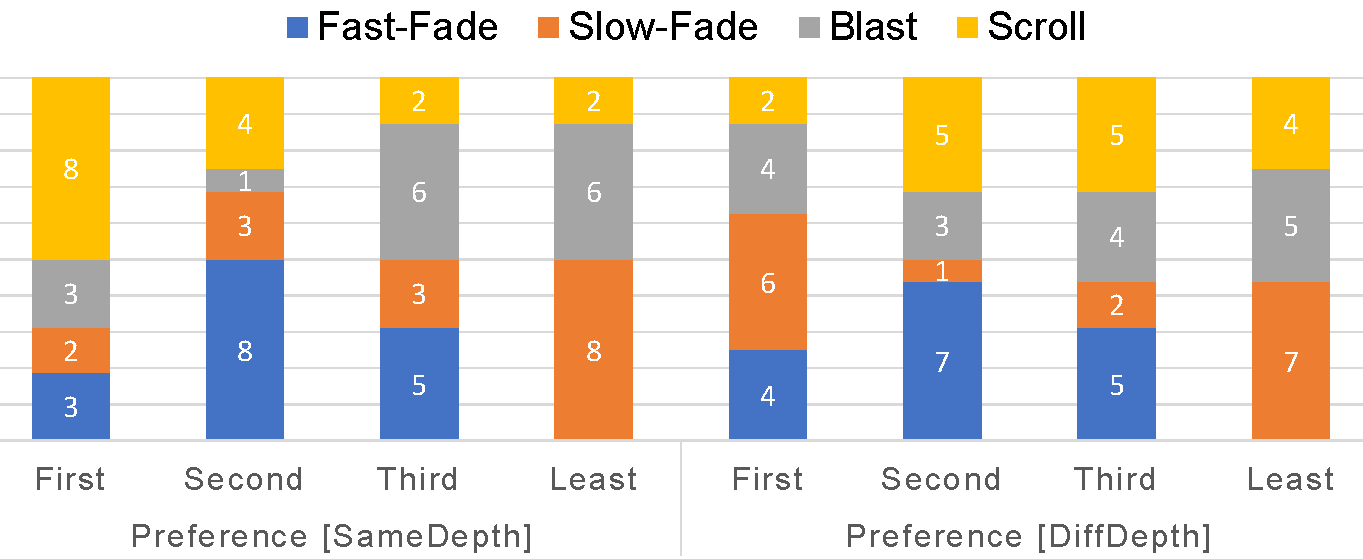
\includegraphics[width=0.85\linewidth]{\Pic{study1/glass_desktop_preference.pdf}}
  \caption[\Animation{} preference in \studyone{}]{\Animation{} preference for OHMD notifications during \glass{} and \desktop{} conditions.}
  \label{fig:GradNotif:study1:preference}
\end{figure}

\autoref{fig:GradNotif:study1:preference} reveals that the majority preferred the \scroll{} \animation{} for \glass{} and \slowfade{} for \desktop{}. However, when taking into account the participants' combined preference choices (for both \glass{} and \desktop{}) and the weighted preference\footnote{\label{footnote:weighted_preference}The weighted preference is determined by assigning weights to each preference and computing their weighted average. For example, the 1st preference is assigned a weight of 4, the 2nd preference a weight of 3, and so on, with the last preference being assigned a weight of 1.} (\autoref{fig:GradNotif:study1:weighted_preference}), the overall tendency favored \fastfade{}. Participants reported that \fastfade{} provided extra preparation time for the secondary task, which allowed faster resumption: \quote{If it's a slow one [\fading{}], I will finish reading the sentence before jumping to notifications. If it's a sudden one [\instant{}, \scroll{}], I will jump to the notification without finishing the sentence}.

\begin{figure}[hptb]
\centering
\begin{subfigure}{\textwidth}
  \centering
  
\includegraphics[width=0.3\linewidth]{\Pic{study1/measure_legends.png}}  
\end{subfigure}
\begin{subfigure}{.4\textwidth}
  \centering
  \includegraphics[width=1\linewidth]{\Pic{study1/measure_weighted_preference.png}}
\end{subfigure}
\caption[Weighted preference in \studyone{}]{Weighted preference$^{\ref{footnote:weighted_preference}}$ (ranking) for each \animation{} with 16 participants. Here, SC = \scroll{}, BL = \instant{}, FF = \fastfade{}, and SF = \slowfade{}. Error bars represent standard error.}
  \label{fig:GradNotif:study1:weighted_preference}	  

\end{figure}

In general, participants preferring \scroll{} found it more noticeable and familiar, remarking it was \quote{very similar to receiving notifications on your phone}. Those favoring \instant{} appreciated the direct display of notifications, enabling them to rapidly attend to notifications and resume proofreading. Conversely, participants who disliked \instant{} or \scroll{} mentioned that these styles were too abrupt, causing distraction from proofreading, with comments such as \quote{I was forced to attend notifications when popping down from [the] top}.

Participants preferring \fading{} felt it provided time to prepare for incoming notifications, cueing them to stop proofreading in advance. Those opposing the \fading{} (primarily \slowfade{}) disliked waiting for notifications as it diverted their attention away from proofreading.

Two participants underscored the importance of context: for urgent notifications, they preferred \scroll{}, whereas, for non-urgent or primary task-unrelated notifications, they favored \fading{}. However, given the maximum delay induced by \fading{} was less than 4 seconds, the \animation{} merely affected perception and did not delay notifications enough to significantly impact.





\subsection{Discussion} 
\label{sec:GradNotif:study1:discussion}
 
This study provides a preliminary understanding of utilizing \fading{} animation in OHMD notifications and the associated trade-offs. 

\subsubsection*{Q1. How does the \fading{} \animation{} compare to blast and scrolling \animation{s}?}

Our results suggest that \fading{} animation reduces interference with the primary task as \readingTime{} was significantly lower than with the \scroll{} animation. Though there appears to be a peak at \fastfade{} in \readingAccuracy{} and an interaction at \fastfade{} for \adjustedReadingAccuracy{}, no statistically significant differences were observed in \readingAccuracy{} or \adjustedReadingAccuracy{}. Thus, \fading{} animation minimizes the primary task interference for task duration but not for accuracy.

While qualitative feedback (\autoref{sec:GradNotif:study1:preference}) indicates that \fading{} minimizes interruptions, no significant differences were noted between \animation{s} in \perceivedInterruption{} or \perceivedTaskLoad{}. Therefore, there is insufficient statistical evidence to argue that \fading{} animation is less distracting and cognitively less demanding than \instant{} or \scroll{}.

Given that there were no significant differences between \animation{s} in \adjustedReadingAccuracy{} and \notificationAccuracy{}, there is insufficient statistical evidence to argue that there is an optimal \fading{} duration. However, according to qualitative feedback, \fadeduration{=2s} (\fastfade{}) allowed participants to prepare for incoming notifications (compared to \fadeduration{=0s}, \instant{}) and minimized the wait for notifications (compared to \fadeduration{=4s}, \slowfade{}), suggesting an optimal \fadeduration{} around 2 seconds. Further studies are required to determine the exact duration.

\subsubsection*{Q2. Does the effect of \fading{} depend on the primary task's \location{}?}

Considering the participants' feedback (\autoref{sec:GradNotif:study1:task_difference}) and the significant main effects of \location{} for \readingTime{}, there is evidence suggesting that interruption due to OHMD notification will be lower for task duration but not accuracy when the notifications are presented at the same depth as the primary task. Nevertheless, further studies are necessary to isolate the effect of location, as the complexity of the primary task confounds the current results. For instance, in the \glass{} condition, users had to scroll through the passage, while in the \desktop{} condition, users did not. This affected the switching between notifications and proofreading (\autoref{sec:GradNotif:study1:task_difference}). Finally, given the lack of significant main or interaction effects in \adjustedReadingAccuracy{}, there is insufficient statistical evidence to either support or refute that the optimal \fading{} duration depends on the primary task's location.



























\section{Study 2: Effects of mobility on \fading{} OHMD notifications}
\label{sec:GradNotif:study2}

This study complements \studyone{} by considering the effects of mobility on \fading{} \animation{}. All other aspects of the procedure were the same as those in \studyone{} (\autoref{sec:GradNotif:study1}), except the apparatus for proofreading, which changed from a desktop to an OHMD (\autoref{sec:GradNotif:study2:apparatus}).

\subsection{Goals}

\i{Q3. Does the effect of \fading{} depend on user \mobility{}?}
In a realistic situation, OHMD users will receive notifications while in stationary and mobile settings. As mobile activities require users to pay additional attention to their physical environment, task complexity tends to increase \cite{oulasvirta_interaction_2005, bailey_effects_2001}. This, in turn, may affect the perception of \fading{} animation. 


\subsection{Participants}
\label{sec:GradNotif:study2:participants}
Sixteen volunteers (10 females, 6 males, age \meansd{22.1}{2.8}) participated in the study. They had similar backgrounds to participants from \studyone{} (\autoref{sec:GradNotif:study1:participants}), except for two participants who had previously used an OHMD for 1 hour.  


\subsection{Apparatus}
\label{sec:GradNotif:study2:apparatus}

In controlled lighting, when OHMD users walk indoors, the focus of their eyes changes based on the distance to obstacles (e.g., walls), which affects the OHMD content display (e.g., the 2D text size can change in OHMDs) \cite{hua_enabling_2017, marran_multiaccomodative_1997}. To eliminate this unwanted effect and simulate a realistic walking experience for mobile conditions \cite{barnard_empirical_2005}, participants were asked to walk on a treadmill (\walking{}, \autoref{fig:GradNotif:study2:apparatus}) at a fixed speed of 2.5 km/h, similar to previous notification evaluations \cite{roumen_notiring_2015, je_pokering_2018}. A black screen around 1m in front of the OHMD was maintained to provide a uniform color projecting surface. For the stationary condition (\sitting{}), participants sat on a chair and attended to tasks similar to \studyone{} (\autoref{fig:GradNotif:study1:apparatus_glass}).

\begin{figure}[hptb]
\centering

\begin{subfigure}{.7\textwidth}
  \centering
  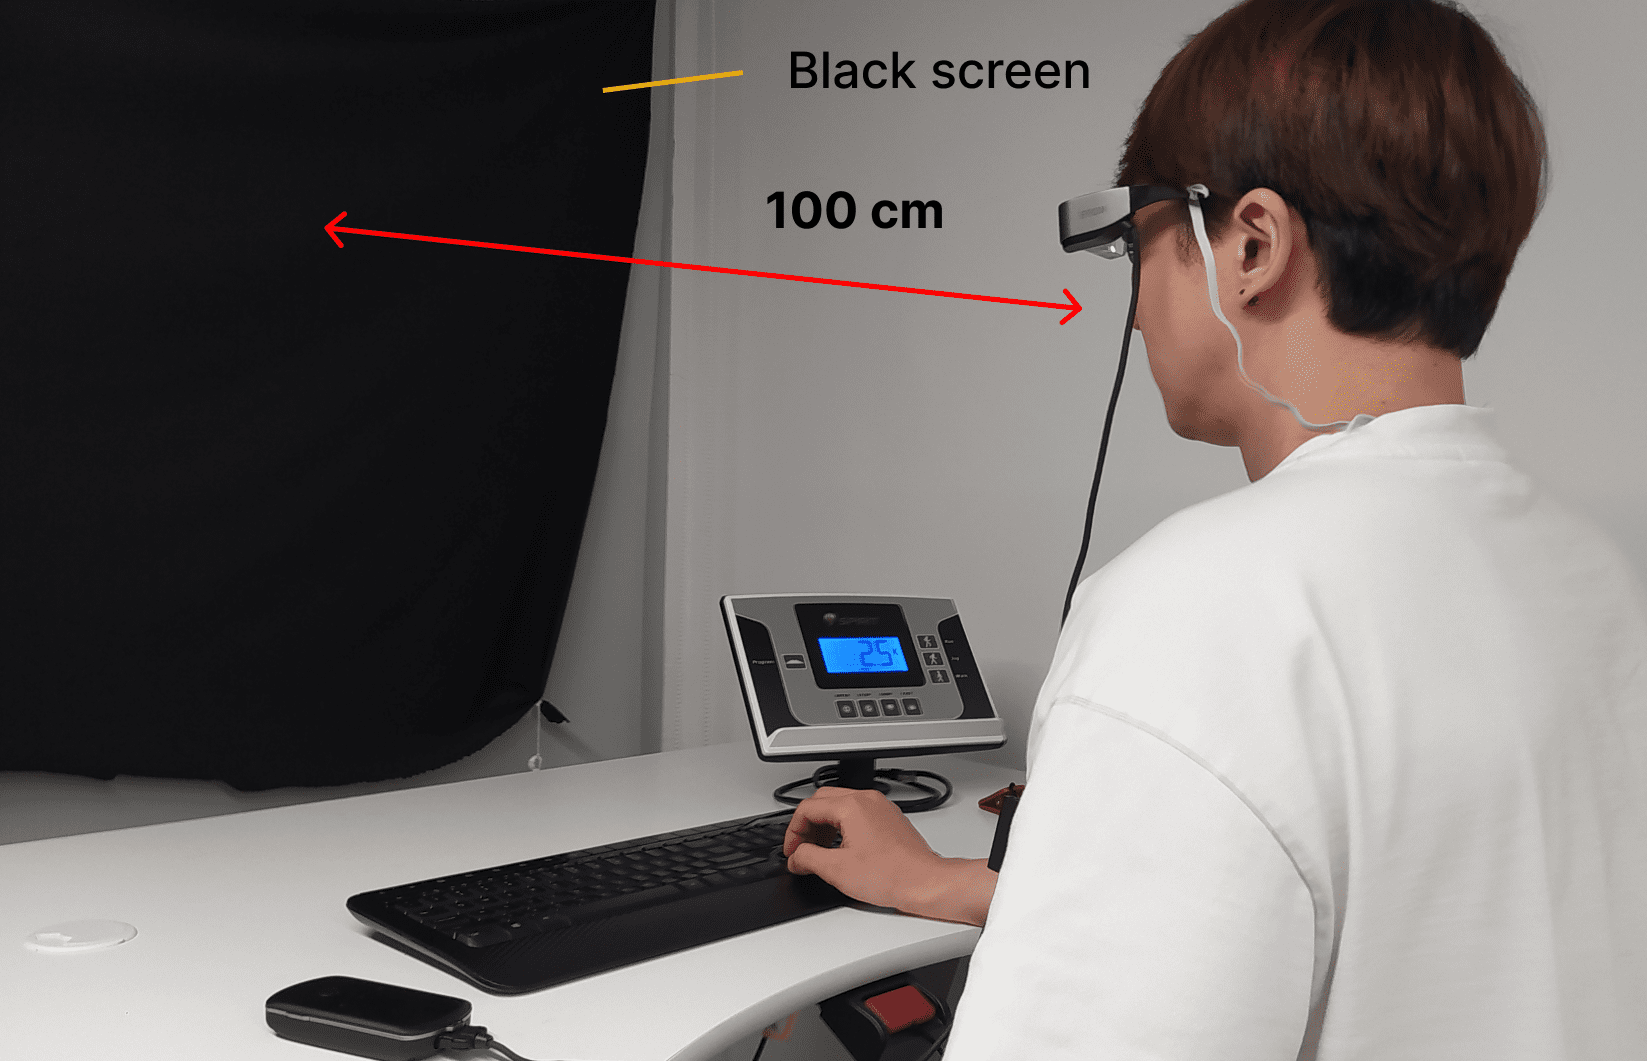
\includegraphics[width=0.98\linewidth]{\Pic{study2/apparatus_mobile_walking1.png}}
  \caption{User controls passages}	  
\end{subfigure}%
\begin{subfigure}{.3\textwidth}
  \centering
  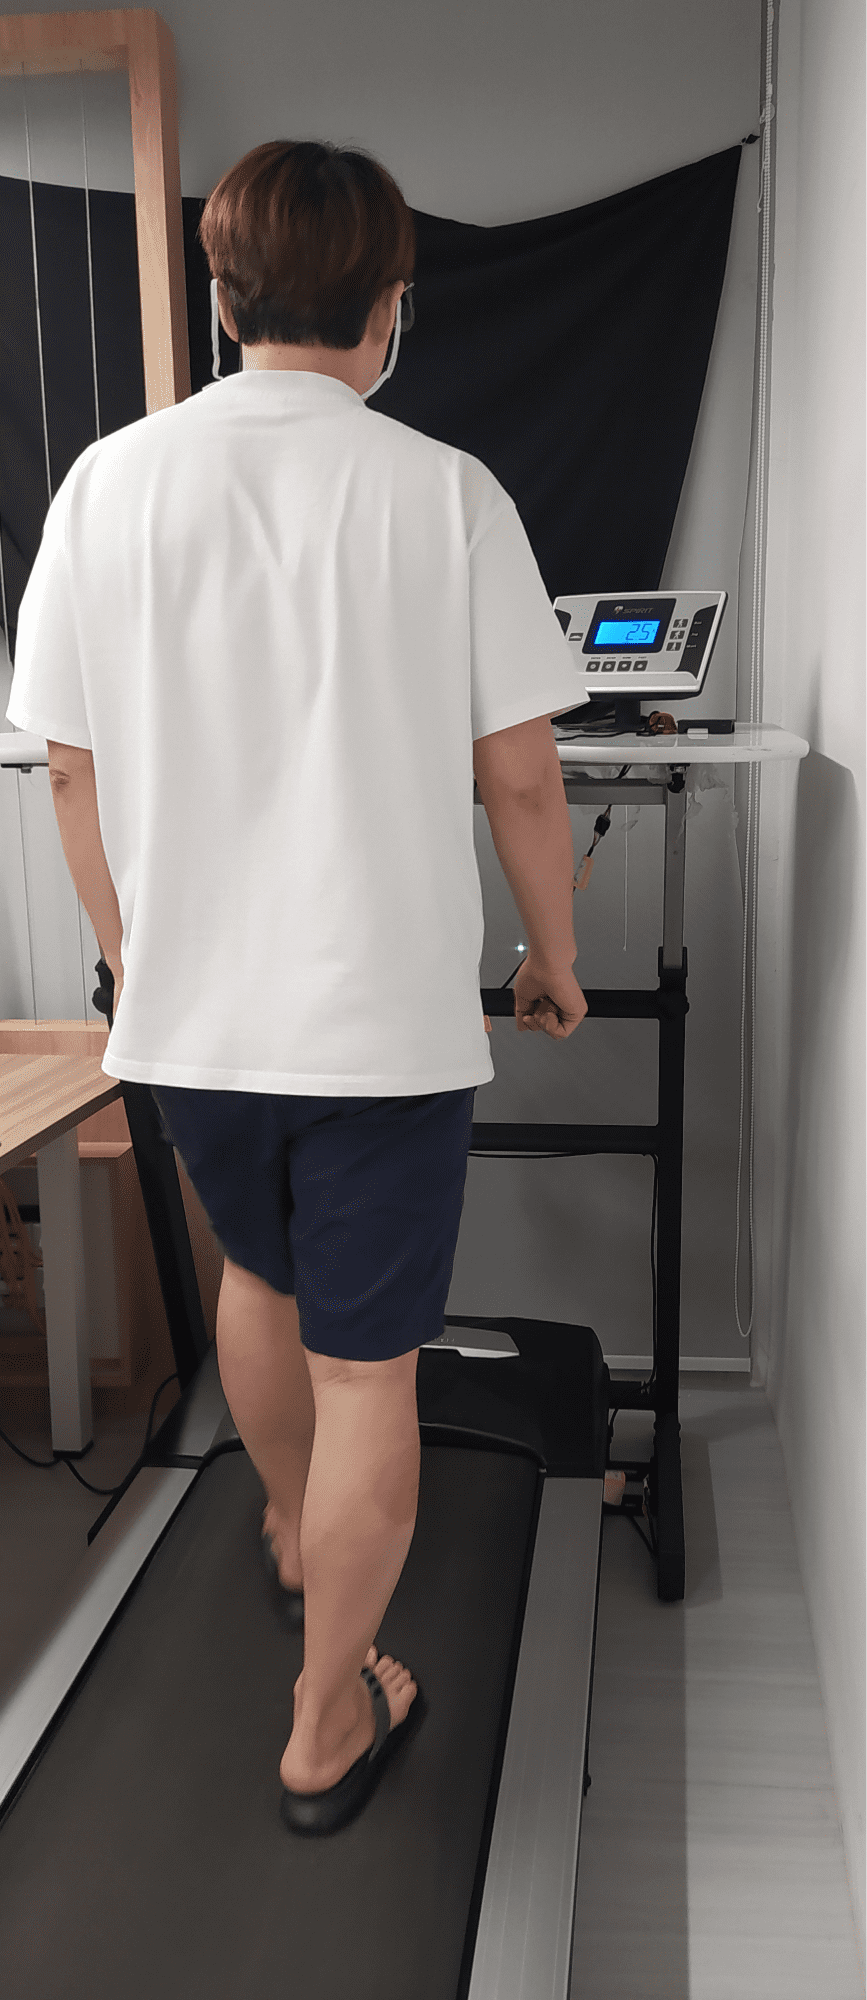
\includegraphics[width=0.63\linewidth]{\Pic{study2/apparatus_mobile_walking2.png}}
  \caption{User walks on treadmill}	  
\end{subfigure}

\caption[Apparatus in \studytwo{}]{Apparatus in mobile (\walking{}) condition.}
\label{fig:GradNotif:study2:apparatus}
\end{figure}


\subsection{Design and procedure}
\label{sec:GradNotif:study2:design_procedure}

A repeated-measures within-subject design was employed to investigate the effects of notifications for two mobility settings (\mobility{}: \sitting{} and \walking{}) and four notification animations (\animation{}: \instant{}, \fastfade{}, \slowfade{}, and \scroll{}). The conditions were counterbalanced using a Latin square blocked by \mobility{} (i.e., half of the participants completed \sitting{} first, while the rest completed \walking{} first) and then \animation{}. 


\subsection{Results}

Each participant completed eight (testing) proofreading tasks and received at least 64 notifications, leading to the collection of 128 data points. \autoref{tab:GradNotif:study2:mean_results}, \autoref{fig:GradNotif:study2:measures_primary_task}, \autoref{fig:GradNotif:study2:measures_task_load}, and \autoref{fig:GradNotif:study2:measures_secondary_task} display the participants' mean performance. 


\begin{table}[hptb]
\centering
\caption[Average performance in \studytwo{}]{Average performance (\i{`mean (sd)'}) in \studytwo{} with 16 participants. The first column represent the  \mobility{}-\animation{} combination using the first letters of each (S = \sitting{}, W = \walking{}; SC = \scroll{}, BL = \instant{}, FF = \fastfade{}, SF = \slowfade{}).}
\label{tab:GradNotif:study2:mean_results}
\scalebox{0.87}{
\begin{tabular}{@{}lp{1.6cm}p{1.9cm}p{1.65cm}p{1.65cm}p{1.8cm}p{1.6cm}p{1.6cm}p{1.6cm}@{}}
\toprule
     & \multicolumn{3}{c}{Primary (reading) task performance}            & \multicolumn{5}{l}{| Secondary (notification) task performance}  \\ \midrule
     & \readingTime{} & \readingAccuracy{} & \adjustedReadingAccuracy{} & \notificationAccuracy{} & \i{Understand-ability} & \i{Notice-ability} & \perceivedInterruption{}     & \perceivedTaskLoad{}     \\ \midrule
S-SC & 169.6 (44.3) & 0.915 (0.102) & 0.573 (0.155) & 0.770 (0.101) & 4.13 (1.50) & 5.13 (1.41) & 57.2 (22.1) & 41.4 (16.8) \\

S-BL & 171.1 (45.1) & 0.920 (0.114) & 0.563 (0.119) & 0.727 (0.129) & 4.50 (1.41) & 5.63 (1.20) & 53.6 (20.6) & 39.5 (13.3) \\

S-FF & 173.2 (48.8) & 0.881 (0.118) & 0.544 (0.162) & 0.770 (0.106) & 4.56 (1.41) & 5.06 (1.44) & 51.9 (22.1) & 38.3 (14.0) \\

S-SF & 173.1 (40.4) & 0.926 (0.101) & 0.555 (0.105) & 0.750 (0.121) & 4.69 (1.30) & 4.88 (1.54) & 53.4 (23.8) & 38.5 (14.8) \\ 
\midrule

W-SC & 191.6 (44.1) & 0.881 (0.118) & 0.482 (0.122) & 0.785 (0.131) & 4.13 (1.67) & 5.31 (1.20) & 63.9 (20.0) & 49.7 (12.4) \\

W-BL & 189.5 (39.9) & 0.909 (0.081) & 0.497 (0.097) & 0.727 (0.137) & 4.50 (1.32) & 5.00 (1.41) & 63.1 (19.9) & 47.3 (15.2) \\

W-FF & 188.8 (46.8) & 0.875 (0.136) & 0.481 (0.096) & 0.777 (0.121) & 4.63 (1.20) & 4.88 (1.63) & 60.9 (20.4) & 47.3 (15.8) \\

W-SF & 186.0 (37.3) & 0.926 (0.101) & 0.512 (0.089) & 0.758 (0.127) & 4.81 (1.42) & 4.88 (1.31) & 62.1 (22.8) & 46.1 (16.4) \\ 
\bottomrule
\end{tabular}
}
\end{table}



\subsection{Primary (reading) task performance}
\label{sec:GradNotif:study2:results_primary_task}

Overall, we observed significant (\pbonf{<0.05}) differences in \readingTime{} and \adjustedReadingAccuracy{}, but no significant differences in \readingAccuracy{}.

\begin{figure*}[hptb]
\centering
\begin{subfigure}{\textwidth}
  \centering
  
\includegraphics[width=0.25\linewidth]{\Pic{study2/measure_legends.png}}  
\end{subfigure}
\begin{subfigure}{.33\textwidth}
  \centering
  \includegraphics[width=\linewidth]{\Pic{study2/measure_reading_time.png}}
  \caption{\readingTime{} (seconds)\significantII{}}
  \label{fig:GradNotif:study2:measure_reading_time}	  
\end{subfigure}%
\begin{subfigure}{.33\textwidth}
  \centering
  \includegraphics[width=\linewidth]{\Pic{study2/measure_reading_accuracy.png}}
  \caption{\readingAccuracy{} (0-1)}
  \label{fig:GradNotif:study2:measure_reading_accuracy}
\end{subfigure}%
\begin{subfigure}{.33\textwidth}
  \centering
  \includegraphics[width=\linewidth]{\Pic{study2/measure_adjusted_reading_accuracy.png}}
  \caption{\adjustedReadingAccuracy{}\significantII{}}
  \label{fig:GradNotif:study2:measure_adjusted_reading_accuracy}	  
\end{subfigure}

\caption[Primary task performance in \studytwo{}]{Primary (reading) task performance (N=16). The X-axis represents the \animation{}, where SC = \scroll{}, BL = \instant{}, FF = \fastfade{}, and SF = \slowfade{}. \significantII{} represents a significant main effect of \mobility{} (\pval{<0.05}). Error bars represent standard error. See \autoref{tab:GradNotif:study2:mean_results} for details.}
\label{fig:GradNotif:study2:measures_primary_task}
\end{figure*}


\begin{itemize}
    \item \readingTime{}: A repeated-measures ANOVA on \readingTime{} revealed a significant main effect of \mobility{} (\anovawefp{1}{15}{12.031}{=0.003}{0.445}), but no significant main effect of \animation{} or interaction effect. Post-hoc analysis (\autoref{fig:GradNotif:study2:measure_reading_time}) revealed that reading while \sitting{} (\meansd{173.73}{43.70}) took significantly (\pbonf{=0.003}, \effd{0.396}) less time than \walking{} (\meansd{188.96}{41.22}).

    \item \readingAccuracy{}: There were no significant main or interaction effects (\autoref{fig:GradNotif:study2:measure_reading_accuracy}).

    \item \adjustedReadingAccuracy{}: A repeated-measures ANOVA showed a significant main effect of \mobility{} (\anovawefp{1}{15}{16.575}{=0.001}{0.525}), but no significant main effect of \animation{} or interaction effect. Post-hoc analysis (\autoref{fig:GradNotif:study2:measure_adjusted_reading_accuracy}) revealed that reading while \sitting{} (\meansd{0.559}{0.134}) enabled significantly (\pbonf{=0.001}, \effd{0.545}) higher accuracy than \walking{} (\meansd{0.493}{0.100}).
    
\end{itemize}


\subsubsection*{Differences between \sitting{} vs. \walking{} conditions}
\label{sec:GradNotif:study2:task_difference}

During post-interviews, all participants reported that proofreading while \walking{} was more difficult and time-consuming than \sitting{} due to the increase in task complexity, even though the walking speed was \quote{average} or \quote{a bit slow}. Walking required additional focus to maintain speed, which reduced the focus on the proofreading task compared to sitting. Moreover, while walking, the OHMD moved along with head movement, making it harder for participants to focus on proofreading and identify the location where they last stopped after attending to notifications.



\subsection{Secondary (notification) task performance}
\label{sec:GradNotif:study2:results_secondary_task}

Overall, no significant main effect of \animation{} on either \Interruption{} or \Reaction{} measures was observed. However, both \Comprehension{} and \Satisfaction{} showed a tendency towards the \fading{} \animation{}.

\subsubsection*{\Interruption{}}
\Animation{} had no significant main effect overall. 

\begin{itemize}
    \item \perceivedInterruption{}: A repeated-measures ANOVA after ART revealed a significant main effect of \mobility{} (\anovawefp{1}{105}{17.394}{<0.001}{0.226}), but no significant main effect of \animation{} or interaction effect was detected. Post-hoc analysis (\autoref{fig:GradNotif:study2:measure_perceived_interruption}) revealed that \perceivedInterruption{} for \walking{} (\meansd{62.53}{20.35}) was significantly higher (\pbonf{<0.05}) than for \sitting{} (\meansd{54.03}{21.75}).
    \item \perceivedTaskLoad{}: A repeated-measures ANOVA revealed a significant main effect of \mobility{} (\anovawefp{1}{15}{13.817}{=0.002}{0.479}), but no significant main effect of \animation{} or interaction effect. Post-hoc analysis revealed that \perceivedInterruption{} for \walking{} (\meansd{47.62}{14.73}) was significantly higher (\pbonf{=0.002}, \effd{0.550}) than that for \sitting{} (\meansd{39.41}{14.49}). Furthermore, \autoref{fig:GradNotif:study2:measure_rtlx} shows a decrease in task load when \fadeduration{} increases from 0 to 4 seconds for both \mobility{} conditions.
\end{itemize}


\begin{figure*}[hptb]
\centering
\begin{subfigure}{\textwidth}
  \centering
  
\includegraphics[width=0.25\linewidth]{\Pic{study2/measure_legends.png}}  
\end{subfigure}
\begin{subfigure}{.45\textwidth}
  \centering
  \includegraphics[width=0.85\linewidth]{\Pic{study2/measure_perceived_interruption.png}}
  \caption{\perceivedInterruption{} (0-100)\significantII{}}
  \label{fig:GradNotif:study2:measure_perceived_interruption}	  
\end{subfigure}%
\begin{subfigure}{.45\textwidth}
  \centering
  \includegraphics[width=0.85\linewidth]{\Pic{study2/measure_rtlx.png}}
  \caption{\perceivedTaskLoad{} (0-100)\significantII{}}
  \label{fig:GradNotif:study2:measure_rtlx}	  
\end{subfigure}

\caption[Secondary task performance (\Interruption{}) in \studytwo{}]{Secondary (notification) task performance on \Interruption{}. The X-axis represents the \animation{}, where SC = \scroll{}, BL = \instant{}, FF = \fastfade{}, and SF = \slowfade{}. \significantII{} represents a significant main effect of \mobility{} (\pval{<0.05}). Error bars represent standard error. See \autoref{tab:GradNotif:study2:mean_results} for details.}
\label{fig:GradNotif:study2:measures_task_load}
\end{figure*}

\subsubsection*{\Reaction{}}

No significant main or interaction effects were found for \noticeability{}. As expected, \autoref{fig:GradNotif:study2:measure_noticeability} demonstrates a decrease in \noticeability{} when \fadeduration{} increased from 0 to 4 seconds for both \location{s}.

\begin{figure*}[hptb]
\centering
\begin{subfigure}{\textwidth}
  \centering
  
\includegraphics[width=0.25\linewidth]{\Pic{study2/measure_legends.png}}  
\end{subfigure}
\begin{subfigure}{.33\textwidth}
  \centering
  \includegraphics[width=\linewidth]{\Pic{study2/measure_noticeability.png}}
  \caption{\noticeability{} (1-7)}
  \label{fig:GradNotif:study2:measure_noticeability}	  
\end{subfigure}%
\begin{subfigure}{.33\textwidth}
  \centering
  \includegraphics[width=\linewidth]{\Pic{study2/measure_undersandability.png}}
  \caption{\understandability{}\significantI{}}
  \label{fig:GradNotif:study2:measure_understandability}
\end{subfigure}%
\begin{subfigure}{.33\textwidth}
  \centering
  \includegraphics[width=\linewidth]{\Pic{study2/measure_notification_accuracy.png}}
  \caption{\notificationAccuracy{} (0-1)}
  \label{fig:GradNotif:study2:measure_notification_accuracy}	  
\end{subfigure}

\caption[Secondary task performance (\Reaction{} and \Comprehension{}) in \studytwo{}]{Secondary (notification) task performance on \Reaction{} and \Comprehension{} (N=16). The X-axis represents the \animation{}, where SC = \scroll{}, BL = \instant{}, FF = \fastfade{}, and SF = \slowfade{}. \significantI{} represents a significant main effect of \animation{} (\pval{<0.05}). Error bars represent standard error. See \autoref{tab:GradNotif:study2:mean_results} for details.}
\label{fig:GradNotif:study2:measures_secondary_task}
\end{figure*}

\subsubsection*{\Comprehension{}}

\autoref{fig:GradNotif:study2:measure_understandability} and \autoref{fig:GradNotif:study2:measure_notification_accuracy} reveal an increase in \understandability{} and \notificationAccuracy{} with \fading{}.

\begin{itemize}
    \item \understandability{}: A repeated-measures ANOVA after ART demonstrated a significant main effect of \animation{} (\anovawefp{3}{105}{3.166}{=0.028}{0.216}), but no significant main effect of \mobility{} or interaction effect. Post-hoc analysis revealed that \understandability{} for \slowfade{} (\meansd{4.75}{1.34}) was significantly higher (\pbonf{<0.05}) than that for \scroll{} (\meansd{4.13}{1.56}). As shown in \autoref{fig:GradNotif:study2:measure_understandability}, \understandability{} increases when \fadeduration{} rises from 0 to 4 seconds for both \mobility{} conditions. This could be because, with \fading{}, users tend to shift their attention to notifications when they anticipate their appearance, as opposed to immediate appearance animations (e.g., \scroll{}, \instant{}) that capture attention instantly.
    \item \notificationAccuracy{}: No significant main or interaction effects were detected (\autoref{fig:GradNotif:study2:measure_notification_accuracy}).
\end{itemize}


\subsubsection*{\Satisfaction{}}
\label{sec:GradNotif:study2:preference}

During the session, twelve participants (\participantproportion{12}{16}) correctly discerned between \animation{s}; however, only one participant (\participantproportion{1}{12}) recognized the differences between \fastfade{} and \slowfade{}. 

\begin{figure}[hptb]
  \centering
  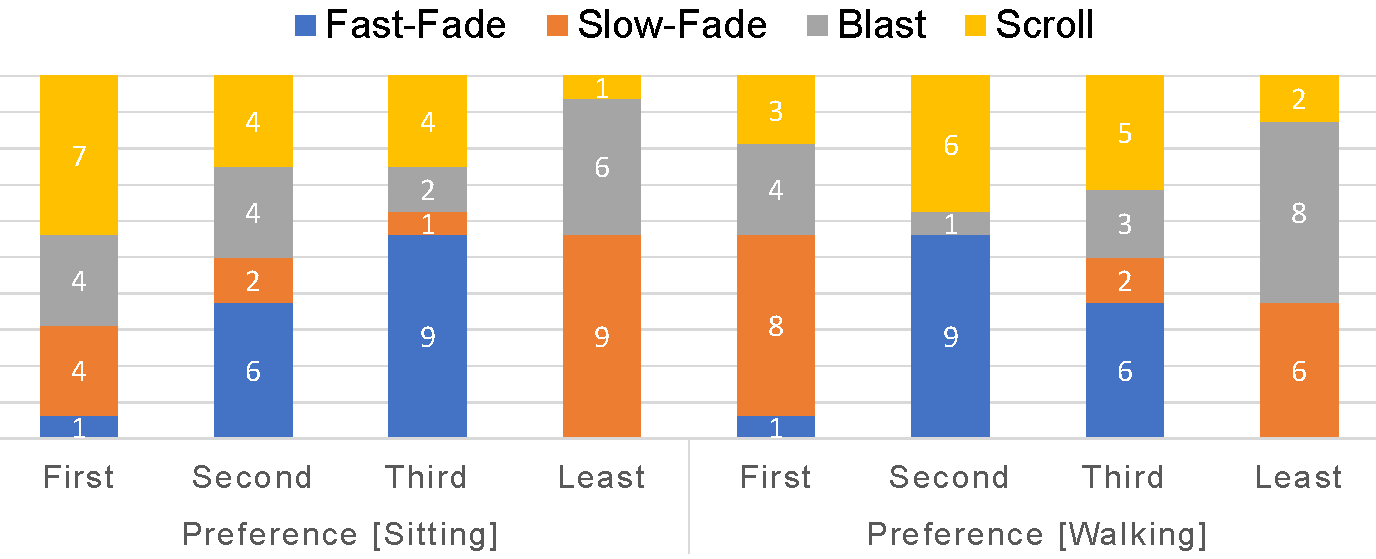
\includegraphics[width=0.85\linewidth]{\Pic{study2/sitting_walking_preference.pdf}}
  \caption[\Animation{} preference in \studytwo{}]{\Animation{} preference for OHMD notifications during \sitting{} and \walking{} conditions.}
  \label{fig:GradNotif:study2:preference}
\end{figure}

As shown in \autoref{fig:GradNotif:study2:preference}, the majority preferred the \scroll{} \animation{} for \sitting{} and \slowfade{} for \walking{}. This preference is also reflected in the weighted preference\footnote{When calculating the weighted preference, both \fastfade{} and \slowfade{} are considered as types of \fading{}.} (\autoref{fig:GradNotif:study2:weighted_preference}), as \fading{} provides users with extra time to prepare for the secondary task, thereby allowing them to resume faster: \quote{I prefer the fade in ones, as it's much easier, and on concentration as well. Because you know, it will appear in a few seconds, and you know something is coming.} The reasons for individual \animation{} preferences were the same as those in \studyone{}, \autoref{sec:GradNotif:study1:preference}. Overall, when task complexity increased, participants preferred \fading{}, particularly \slowfade{}, for \walking{}, mirroring the results from \studyone{}.

\begin{figure}[hptb]
\centering
\begin{subfigure}{\textwidth}
  \centering
  
\includegraphics[width=0.25\linewidth]{\Pic{study2/measure_legends.png}}  
\end{subfigure}
\begin{subfigure}{.40\textwidth}
  \centering
  \includegraphics[width=1\linewidth]{\Pic{study2/measure_weighted_preference.png}}
\end{subfigure}
\caption[Weighted preference in \studytwo{}]{Weighted preference (ranking) for each \animation{} with 16 participants. Here, SC = \scroll{}, BL = \instant{}, FD = \fading{} (taken \fastfade{} and \slowfade{} together). Error bars represent standard error.}
  \label{fig:GradNotif:study2:weighted_preference}	  

\end{figure}









\subsection{Discussion} 
\label{sec:GradNotif:study2:discussion}

This study provides an initial understanding of how mobility affects the usage of \fading{} animation in OHMD notifications. 

\subsubsection*{Q3. Does the effect of \fading{} depend on user \mobility{}?}

Although there was no statistically significant difference in \readingTime{} or \adjustedReadingAccuracy{} (\autoref{sec:GradNotif:study2:results_primary_task}), the study results suggest that \fading{} animation reduces interference with the primary task during the \walking{} condition, as also backed by qualitative feedback (\autoref{fig:GradNotif:study2:preference}). However, the results also show that \perceivedTaskLoad{} decreases and \understandability{} significantly increases when \fadeduration{} increases (\autoref{sec:GradNotif:study2:results_secondary_task}).
Comparing \sitting{} vs. \walking{} conditions, these results indicate that the effect of \fading{} (e.g., \Interruption{}, \Reaction{}, and \Comprehension{}), indeed, depends on \mobility{}; and when task complexity increases, \fading{} can improve \Comprehension{} and reduce \Interruption{} with no significant effect on \Reaction{}.
















\section{General discussion}
\label{sec:GradNotif:general_discussion}

As indicated in \autoref{sec:GradNotif:study1:results_secondary_task} and \autoref{sec:GradNotif:study2:results_secondary_task}, \fading{} animation performs comparably to \instant{} and \scroll{} in \Reaction{} and \Comprehension{}. Furthermore, \fading{} animation can mitigate the interference with primary tasks and \Interruption{}, providing users with an opportunity to prepare for upcoming notifications. 

This result can be explained using the Unified Multitasking Theory \cite{salvucci_toward_2009} (\autoref{fig:Relatedwork:interruption_resumption}). \Fading{} animation provides an interruption lag (with the \fadeduration{}), allowing participants to remember the state of the primary task before attending to notifications. This subsequently facilitates faster resumption of the primary task by reducing the resumption lag associated with recalling where participants paused the primary task. However, the benefits of \fading{} animation are contingent on its \fadeduration{}, location, and the complexity of the primary task (\autoref{sec:GradNotif:study1:task_difference}, \autoref{sec:GradNotif:study2:task_difference}). If the \fadeduration{} is too short, \fading{} animation can draw attention to the notification too abruptly, disrupting the primary task. Conversely, if the \fadeduration{} is too long, users might have to wait excessively before notifications become legible, which also interrupts the primary task.

Furthermore, the \fading{} animation aids users in preparing for focus shifts between the OHMD notifications and their non-OHMD primary tasks, accommodating different task locations. Similarly, as the complexity of the primary task increases, the interruption caused by notifications escalates \cite{bailey_effects_2001, borst_what_2015}; hence, \fading{} animation that offers sufficient interruption lag to remember the state of the primary task minimizes this interruption. Consequently, the optimal \fadeduration{} duration depends on the complexity of the task (\autoref{sec:GradNotif:study1:discussion}, \autoref{sec:GradNotif:study2:discussion}).

As anticipated, notifications become less noticeable when the \fadeduration{} increases. Given that the lighting of the external environment influences the noticeability of OHMD content \cite{erickson_exploring_2020}, the optimal \fadeduration{} also depends on external lighting. Thus, both \fadeduration{} and OHMD display brightness should dynamically adjust to the user's lighting conditions.

Although \fading{} animation can mitigate the interference with primary tasks, its practical use should depend on the utility of notifications \cite{mccrickard_attuning_2003, gluck_matching_2007}. As expressed by several participants (\autoref{sec:GradNotif:study1:preference}), how notifications appear can signal their importance and urgency levels; slow \fading{} notifications are well-suited to signal lower levels of urgency \cite{faulhaber_priority_dependent_2022}. Although perceived urgency and importance are influenced by \fadeduration{}, the maximum delay for notifications was 4 seconds. This implies that \fadeduration{} is not the predominant factor affecting attendance to notifications.

Given that the features used in our OHMD prototype are a subset of those from advanced OHMDs (e.g., Microsoft HoloLens) supporting a wider field-of-view and various anchoring techniques (e.g., world anchoring), we believe that our results can be replicated in advanced OHMDs using similar configurations \cite{janaka_can_2023}.

Finally, this study employed text reading, a structured visual search task, which lacks support for resumability \cite{smith_visual_2015}. Thus, the results can be applied to similar tasks such as browsing, gaming, and driving. However, if the primary task supports resumability (e.g., grid searching), \fading{} may not have an advantage over other animations in terms of task performance.







\section{Limitations}
\label{sec:GradNotif:limitations}

In this study, 5-word single-color text notifications were used to isolate the effect of animation. However, real notifications contain additional elements such as colors, icons, and multiple text content \cite{android_android_2021} that can impact the effects of \fading{} \cite{luyten_hidden_2016, bailey_effects_2001}, necessitating further exploration. 
Although subjective ratings with a 2-second interval provided an initial understanding of \fadeduration{}, more granular details could be obtained using eye-tracking and finer intervals (e.g., 1, 0.5 seconds). 
Since the notification duration was fixed (i.e., 10s), the \fadeduration{} influenced the time available for reading notifications, potentially affecting the interference with the primary task \cite{monk_effect_2008}. 
However, participant feedback indicated that they did not read notifications even when they appeared for longer periods (e.g., \instant{}), suggesting that the results were not influenced by the available time.


\section{Programming codes}
\label{sec:GradNotif:programming_codes}

\begin{sloppypar}
The codes for this study can be found at \url{https://github.com/NUS-HCILab/FadingNotifications}. 
\end{sloppypar}

\section{Conclusion}

Through two controlled studies, we determined that \fading{} animations can minimize the interference of OHMD notifications with primary tasks compared to the prevalent \instant{} and \scroll{} animations. Furthermore, we found that the effectiveness of \fading{} animations depends on \fadeduration{}, the location of the primary task (i.e., depth), and the complexity of the primary task (e.g., mobility). The results suggest that the optimal \fadeduration{} is influenced by the complexity of the primary task and is approximately 2-4 seconds for reading tasks; this needs further examination.

Future research could investigate the design of an adaptive notification system for OHMDs in which the animation and its properties (e.g., fade-duration for fading, scroll-duration for scrolling) are dynamically altered based on the user context (e.g., brightness of the environment), the primary task (e.g., mobile reading), and the message content (e.g., importance or urgency of the notification) to deliver notifications that align with user expectations (e.g., minimize distractions).

Given these results, this chapter provides an answer to our thesis question (\autoref{sec:Intro:thesis_RQ}). We can effectively reduce the attention costs associated with OHMD notifications during multitasking by presenting information gradually, such as with fading animations, to enable quick resumption of primary tasks.

\subsubsection*{Summary of statistically significant results:}
{\small
\begin{itemize}
    \item In the stationary (lab) setting, 
    \begin{itemize}
        \item Attending to notifications at the same location (i.e., depth) as the primary task resulted in reduced primary task completion time (i.e., reading time) and perceived interruption compared to when the tasks were at different locations.
        \item \Slowfade{} animations required less time to complete the primary task than \scroll{} animations.
        \item When tasks were at the same location, the majority of participants (50\%) ranked \scroll{} as their first preference. Similarly, at different locations, the majority (38\%) ranked \slowfade{} as their first preference.
    \end{itemize}
    \item In the mobile (lab) setting, 
    \begin{itemize}
        \item While sitting, the primary task completion time was less than when walking.
        \item While sitting, the primary task accuracy was higher than when walking.
        \item While sitting, both the perceived interruption and task load were lower than when walking.
        \item \Slowfade{} animations were perceived as more understandable than \scroll{} animation.
        \item While sitting, the majority of participants (44\%) ranked \scroll{} as their first preference. Similarly, while walking, the majority (50\%) ranked \slowfade{} as their first preference.
    \end{itemize}
\end{itemize}
}